\documentclass[answers]{exam}

\usepackage{amsmath, amsfonts, amssymb}
\usepackage{geometry}
\usepackage{graphics}
\usepackage{graphicx}
\usepackage{tikz}
\usepackage{listings}
% \usepackage{subfig}
\usepackage{float}

\lstset{
    basicstyle=\ttfamily,
    columns=fullflexible,
    frame=single,
    breaklines=true,
    postbreak=\mbox{\textcolor{red}{$\hookrightarrow$}\space},
}

\geometry{
    bottom=2cm, % Adjust this value as needed to leave space for the answer boxes
}

% Header and footer.
\pagestyle{headandfoot}
\runningheadrule
\runningfootrule
\runningheader{EE/CE 468/468 Mobile Robotics}{Homework 3}{Fall 2023}
\runningfooter{}{Page \thepage\ of \numpages}{}
\firstpageheader{}{}{}

\boxedpoints
\printanswers

\newcommand{\uvec}[1]{\boldsymbol{\hat{\textbf{#1}}}}
\newcommand\union\cup
\newcommand\inter\cap
\newcommand\ul\underline
\newcommand\ol\overline

\title{Assignment 3\\ EE/CE 468/468 Mobile Robotics\\ Habib University -- Fall 2023}
\author{Ali Asghar Yousuf \\ Muhammad Azeem Haider }
\date{\today}

\begin{document}
\maketitle

\begin{questions}
    \question[20]
    Consider a robot that lives in a 1-D coordinate system. Its location will be denoted by \(x\), its velocity by \(\dot{x}\), and its acceleration by \(\ddot{x}\). Suppose we can only control the acceleration \(\ddot{x}\). Making use of equations of motion from school physics, write the discrete-time motion model for this system. Assume that the acceleration \(\ddot{x}\) is a sum of a commanded acceleration and a zero-mean noise term with variance \(\sigma^2\) and assume that the actual acceleration remains constant in an interval \(\Delta t\).
    \begin{parts}
        \part Find the uncertainty/covariance in the pose \((x, \dot{x})\) after one time step. Are the two correlated?
        \begin{solution}
            Starting with the classic kinematic equations:
            \begin{align*}
                x & = v_i t + \frac{1}{2} a t^2, \\
                v & = v_i + a t,
            \end{align*}
            and transitioning to a discrete-time domain for the \( k \)-th time step, we get:
            \begin{align*}
                x_{k+1}       & = x_k + \dot{x}_k \Delta t + \frac{1}{2} \ddot{x}_k \Delta t^2, \\
                \dot{x}_{k+1} & = \dot{x}_k + \ddot{x}_k \Delta t.
            \end{align*}

            The acceleration includes a deterministic part and a random noise component:
            \begin{align*}
                \ddot{x}_k & = a_k + \eta_k,      \\
                \eta_k     & \sim N(0, \sigma^2).
            \end{align*}

            The state transition incorporating noise becomes:
            \begin{align*}
                x_{k+1}       & = x_k + \dot{x}_k \Delta t + \frac{1}{2} (a_k + \eta_k) \Delta t^2, \\
                \dot{x}_{k+1} & = \dot{x}_k + (a_k + \eta_k) \Delta t.
            \end{align*}

            \[
                \Sigma = \begin{bmatrix}
                    \sigma_{xx}       & \sigma_{x\dot{x}}       \\
                    \sigma_{x\dot{x}} & \sigma_{\dot{x}\dot{x}}
                \end{bmatrix}
            \]
            where:
            \begin{itemize}
                \item \( \sigma_{xx} \) is the variance of the position \( x \),
                \item \( \sigma_{\dot{x}\dot{x}} \) is the variance of the velocity \( \dot{x} \),
                \item \( \sigma_{x\dot{x}} \) is the covariance between position \( x \) and velocity \( \dot{x} \).
            \end{itemize}
            The non-zero \( \sigma_{x\dot{x}} \) implies that the position and velocity are correlated after one time step, influenced by the acceleration noise.
        \end{solution}

        \part Suppose we control this robot with a commanded acceleration sequence \(a_1, a_2, a_3, \ldots\) for \(T\) time intervals. Will the final location \(x\) and the final velocity \(\dot{x}\) be correlated for some large value of \(T\)?
        \begin{solution}
            Over a large number of time intervals \(T\), the final location \(x\) and velocity \(\dot{x}\) will accumulate changes due to the commanded accelerations and noise. As \(T\) increases, the influence of initial conditions on the final state diminishes, and the cumulative effect of accelerations becomes more significant. If the accelerations are uncorrelated over time and the noise is zero-mean, the final position and velocity may become less correlated. However, any patterns or dependencies in the commanded accelerations could induce a correlation between the final position and velocity.
        \end{solution}

    \end{parts}

    \question[20]
    Suppose we have a mobile robot operating in a planar environment. Its state is its \(x\)-\(y\) location and its global heading direction \(\theta\). Suppose we know \(x\) and \(y\) with high certainty but the orientation \(\theta\) is unknown. This is reflected in our initial estimate:
    \[
        \hat{x}_0 = \begin{bmatrix} 0 \\ 0 \\ 0 \end{bmatrix}, \quad
        \Sigma_0 = \begin{bmatrix} 0.01 & 0 & 0 \\ 0 & 0.01 & 0 \\ 0 & 0 & 10000 \end{bmatrix}.
    \]
    \begin{parts}
        \part Assume that the robot moves flawlessly without any noise. We'll consider the simple case when the robot's heading is not being controlled i.e. \(\omega = 0\). Observations of the robot are made at discrete points in time and consist of the robot's distance from the origin \(d\) and the bearing \(\theta\) measured from the origin. Assume that the noise associated with these two measurements are independent. Develop a Kalman Filter that maintains an estimate of the robot’s state.
        \begin{solution}
            % develop a kalman filter instead of an extended kalman filter
            Since the robot's heading is not being controlled and the robot moves
            flawlessly without any noise, the state transition model is given by:
            \begin{align*}
                x_{k+1}      & = x_k + v_k \Delta t \cos(\theta_k),   \\
                y_{k+1}      & = y_k + v_k \Delta t \sin(\theta_k),   \\
                \theta_{k+1} & = \theta_k.                            \\
                A_k          & = \begin{bmatrix}
                                     1 & 0 & -v_k \Delta t \sin(\theta_k) \\
                                     0 & 1 & v_k \Delta t \cos(\theta_k)  \\
                                     0 & 0 & 1
                                 \end{bmatrix} \\
            \end{align*}

            The observation model is given by:
            \begin{align*}
                d_k      & = \sqrt{x_k^2 + y_k^2} + \eta_k,                                              \\
                \theta_k & = \tan^{-1}\left(\frac{y_k}{x_k}\right) + \eta_k.                             \\
                C_k      & = \begin{bmatrix}
                                 \frac{x_k}{\sqrt{x_k^2 + y_k^2}} & \frac{y_k}{\sqrt{x_k^2 + y_k^2}} & 0
                             \end{bmatrix} \\
            \end{align*}

            The state transition noise covariance matrix is given by:
            \begin{align*}
                R_k & = \begin{bmatrix}
                            0 & 0 & 0 \\
                            0 & 0 & 0 \\
                            0 & 0 & 0
                        \end{bmatrix} \\
            \end{align*}

            The observation noise covariance matrix is given by:
            \begin{align*}
                Q_k & = \begin{bmatrix}
                            \sigma^2_{d} & 0                 \\
                            0            & \sigma^2_{\theta}
                        \end{bmatrix}
            \end{align*}

            The Kalman Filter equations are given by:

            \textbf{Prediction Step:}
            \begin{align*}
                \bar{x}_{k}      & = A_{k} \hat{x}_{k-1},       \\
                \bar{\Sigma}_{k} & = A_{k} \Sigma_{k-1} A_{k}^T
            \end{align*}

            \textbf{Update Step:}
            \begin{align*}
                K_{k}       & = \bar{\Sigma}_{k} C_{k}^T \left(C_{k} \Sigma_{k} C_{k}^T + Q_{k}\right)^{-1}, \\
                \hat{x}_{k} & = \bar{x}_{k} + K_{k} \left(z_{k} - C_{k} \bar{x}_{k}\right),                  \\
                \Sigma_{k}  & = \left(I - K_{k} C_{k}\right) \bar{\Sigma}_{k}.
            \end{align*}
        \end{solution}

        \part The location of the robot is a random vector. Draw 1000 samples of the initial state from a Gaussian distribution of the stated mean and covariance, propagate each initial state sample according to the motion equation and plot the samples of the \(x\)-\(y\) state only at time 1 in MATLAB. Assume that distance covered in one time step is 1.
        \begin{solution}
            The following figure shows the 1000 samples of the initial state propagated
            according to the motion equation at time 1.
            \begin{figure}[H]
                \centering
                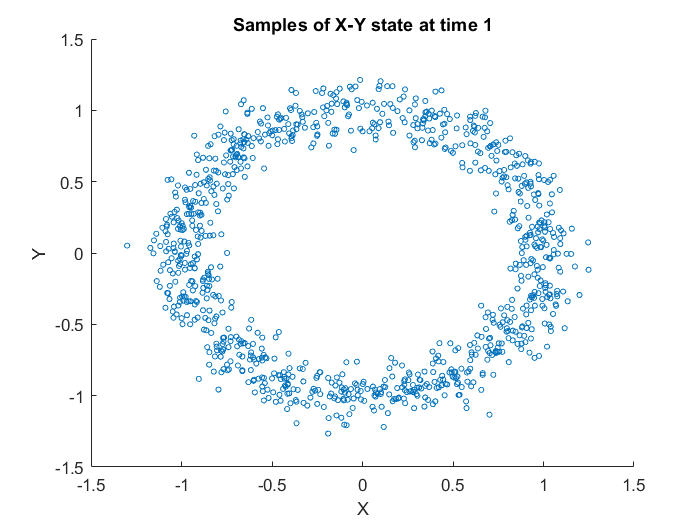
\includegraphics[width=0.8\textwidth]{images/2b.png}
                \caption{1000 samples of the initial state propagated according to the motion equation at time 1.}
            \end{figure}
        \end{solution}

        \part Use the prediction step of the EKF to make a prediction about the state at time 1 and its corresponding covariance. Plot the uncertainty ellipse of a Gaussian with mean equal to \(\bar{x}_1\) and covariance \(\bar{\Sigma}_1\) on the same plot as (a) and compare and comment on the two.
        \begin{solution}
            Using the prediction step of the EKF:
            \begin{align*}
                \bar{x}_{k}      & = g(\hat{x}_{k-1}),                            \\
                \bar{\Sigma}_{k} & = G_{k} \Sigma_{k-1} G_{k}^T
                \intertext{where}
                G_{k}            & = \begin{bmatrix}
                                         1 & 0 & -v_{k-1} \Delta t \sin(\theta_{k-1}) \\
                                         0 & 1 & v_{k-1} \Delta t \cos(\theta_{k-1})  \\
                                         0 & 0 & 1
                                     \end{bmatrix} \\
                \Delta t         & = 1                                            \\
                v_0              & = 1                                            \\
                \theta_0         & = 0                                            \\
                \hat{x}_{0}      & = \begin{bmatrix}
                                         0 \\ 0 \\ 0
                                     \end{bmatrix}                               \\
                \Sigma_{0}       & = \begin{bmatrix}
                                         0.01 & 0    & 0     \\
                                         0    & 0.01 & 0     \\
                                         0    & 0    & 10000
                                     \end{bmatrix}                          \\
            \end{align*}

            Putting the values in the above equations, we get:
            \begin{align*}
                \bar{x}_{1}      & = \begin{bmatrix}
                                         \hat{x}_{0} + v_0 \Delta t \cos(\theta_0) \\
                                         \hat{y}_{0} + v_0 \Delta t \sin(\theta_0) \\
                                         \hat{\theta}_{0}
                                     \end{bmatrix}
                = \begin{bmatrix}
                      0 + (1)(1)\cos(0) \\ 0 + (1)(1)\sin(0) \\ 0
                  \end{bmatrix}
                = \begin{bmatrix}
                      1 \\ 0 \\ 0
                  \end{bmatrix},                                                                                                \\
                \bar{\Sigma}_{1} & = \begin{bmatrix}
                                         1 & 0 & -v_0 \Delta t \sin(\theta_0) \\
                                         0 & 1 & v_0 \Delta t \cos(\theta_0)  \\
                                         0 & 0 & 1
                                     \end{bmatrix} \begin{bmatrix}
                                                       0.01 & 0    & 0     \\
                                                       0    & 0.01 & 0     \\
                                                       0    & 0    & 10000
                                                   \end{bmatrix} \begin{bmatrix}
                                                                     1                            & 0                           & 0 \\
                                                                     0                            & 1                           & 0 \\
                                                                     -v_0 \Delta t \sin(\theta_0) & v_0 \Delta t \cos(\theta_0) & 1
                                                                 \end{bmatrix} \\
                                 & = \begin{bmatrix}
                                         1 & 0 & 0 \\
                                         0 & 1 & 1 \\
                                         0 & 0 & 1
                                     \end{bmatrix} \begin{bmatrix}
                                                       0.01 & 0    & 0     \\
                                                       0    & 0.01 & 0     \\
                                                       0    & 0    & 10000
                                                   \end{bmatrix} \begin{bmatrix}
                                                                     1 & 0 & 0 \\
                                                                     0 & 1 & 0 \\
                                                                     0 & 1 & 1
                                                                 \end{bmatrix}                                                 \\
                                 & = \begin{bmatrix}
                                         0.01 & 0     & 0     \\
                                         0    & 10000 & 10000 \\
                                         0    & 10000 & 10000
                                     \end{bmatrix}
            \end{align*}

            The uncertainty ellipse of a Gaussian with mean equal to \(\bar{x}_1\) and
            covariance \(\bar{\Sigma}_1\) is shown in the following figure:
            % \begin{figure}[H]
            %     \centering
            %     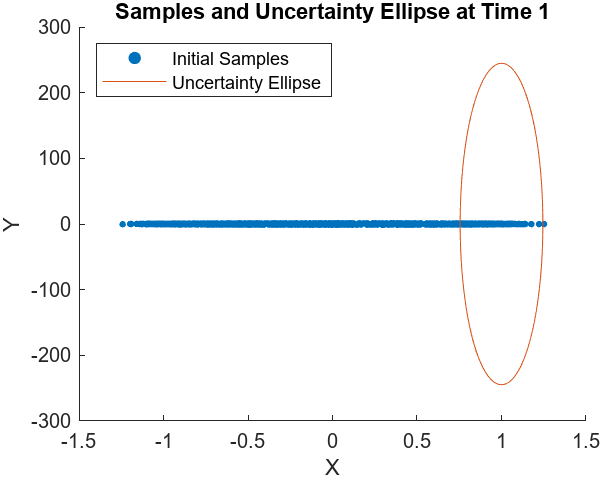
\includegraphics[width=0.8\textwidth]{images/2c.png}
            %     \caption{Uncertainty ellipse of a Gaussian with mean equal to \(\bar{x}_1\) and covariance \(\bar{\Sigma}_1\).}
            % \end{figure}
        \end{solution}

        \part Now incorporate a noisy measurement i.e. \(z = d + \epsilon\) where \(\epsilon\) is zero-mean with covariance 0.01. Again draw the uncertainty ellipse on the same plot after incorporating the measurement.
        \begin{solution}
            The observation model in this problem is given by:
            \begin{align*}
                z_k    & = \sqrt{x_k^2 + y_k^2} + \eta_k                                                 \\
                \eta_k & \sim N(0, \sigma^2)                                                             \\
                \intertext{We know that,}
                z_k    & = h(x_k) + \eta_k                                                               \\
                K_k    & = \bar{\Sigma}_k H_k^T \left(H_k \bar{\Sigma}_k H_k^T + Q_k\right)^{-1}         \\
                \intertext{where}
                H_k    & = \begin{bmatrix}
                               \dfrac{x_k}{\sqrt{x_k^2 + y_k^2}} & \dfrac{y_k}{\sqrt{x_k^2 + y_k^2}} & 0
                           \end{bmatrix} \\
                \intertext{Therefore, we can calculate \(K_k\) as follows:}
                K_1    & = \Sigma_1 H_1^T \left(H_1 \Sigma_1 H_1^T + Q_1\right)^{-1}                     \\
                H_1    & = \begin{bmatrix}
                               \dfrac{1}{\sqrt{1^2 + 0^2}} & \dfrac{0}{\sqrt{1^2 + 0^2}} & 0
                           \end{bmatrix}
                = \begin{bmatrix}
                      1 & 0 & 0
                  \end{bmatrix}
            \end{align*}                                                                                                 \\

            From previous calculation we know that,

            \begin{align*}
                \Sigma_1 & = \begin{bmatrix}
                                 0.01 & 0     & 0     \\
                                 0    & 10000 & 10000 \\
                                 0    & 10000 & 10000
                             \end{bmatrix}                                                                                    \\
                K_1      & = \begin{bmatrix}
                                 0.01 & 0    & 0     \\
                                 0    & 0.01 & 0     \\
                                 0    & 0    & 10000
                             \end{bmatrix} \begin{bmatrix}
                                               1 \\ 0 \\ 0
                                           \end{bmatrix} \left(\begin{bmatrix}
                                                                   1 & 0 & 0
                                                               \end{bmatrix} \begin{bmatrix}
                                                                                 0.01 & 0    & 0     \\
                                                                                 0    & 0.01 & 0     \\
                                                                                 0    & 0    & 10000
                                                                             \end{bmatrix} \begin{bmatrix}
                                                                                               1 \\ 0 \\ 0
                                                                                           \end{bmatrix} + \begin{bmatrix}
                                                                                                               0.01
                                                                                                           \end{bmatrix}\right)^{-1} \\
                         & = \begin{bmatrix}
                                 0.5 \\ 0 \\ 0
                             \end{bmatrix}
            \end{align*}
            For $\hat{x}_1$,
            \begin{align*}
                \hat{x}_1 & = \bar{x}_1 + K_1 \left(z_1 - h(\bar{x}_1)\right)                   \\
                          & = \begin{bmatrix}
                                  1 \\ 0 \\ 0
                              \end{bmatrix} + \begin{bmatrix}
                                                  0.5 \\ 0 \\ 0
                                              \end{bmatrix} \left(z_1 - \sqrt{1^2 + 0^2}\right) \\
            \end{align*}

            $z_1 \sim N(1, 0.01)$, if we put in the mean we get,

            \begin{align*}
                \hat{x}_1 & = \begin{bmatrix}
                                  1 \\ 0 \\ 0
                              \end{bmatrix} + \begin{bmatrix}
                                                  0.5 \\ 0 \\ 0
                                              \end{bmatrix} \left(1 - 1\right)
                = \begin{bmatrix}
                      1 \\ 0 \\ 0
                  \end{bmatrix}
            \end{align*}
            For $\Sigma_1$,
            \begin{align*}
                \Sigma_1 & = \left(I - K_1 H_1\right) \bar{\Sigma}_1                           \\
                         & = \left(I - \begin{bmatrix}
                                               0.5 \\ 0 \\ 0
                                           \end{bmatrix} \begin{bmatrix}
                                                             1 & 0 & 0
                                                         \end{bmatrix}\right) \begin{bmatrix}
                                                                              0.01 & 0     & 0     \\
                                                                              0    & 10000 & 10000 \\
                                                                              0    & 10000 & 10000
                                                                          \end{bmatrix} \\
                         & = \begin{bmatrix}
                                 0.005 & 0     & 0     \\
                                 0     & 10000 & 10000 \\
                                 0     & 10000 & 10000
                             \end{bmatrix}
            \end{align*}
        \end{solution}

        \part What would have been your estimate for the \(x\)-\(y\) at time 1 considering (a)? What would be your comments about the estimate provided by the EKF? What would have happened if the initial orientation were known but we were uncertain about the \(y\) coordinate?
        \begin{solution}
        \end{solution}
    \end{parts}

    \question[20]
    Suppose we live at a place where days are either sunny, cloudy, or rainy. The weather tomorrow is determined solely by the weather today (it’s a Markov Chain) and is captured by the following state transition probabilities:
    \begin{center}
        \textbf{Today's Weather} \\
        \begin{tabular}{|c|c|c|c|}
            \hline
            \textbf{}       & \textbf{Sunny} & \textbf{Cloudy} & \textbf{Rainy} \\ \hline
            \textbf{Sunny}  & 0.8            & 0.2             & 0              \\ \hline
            \textbf{Cloudy} & 0.4            & 0.4             & 0.2            \\ \hline
            \textbf{Rainy}  & 0.2            & 0.6             & 0.2            \\ \hline
        \end{tabular}
    \end{center}
    Suppose that we cannot observe the weather directly but instead rely on a sensor. Our sensor is noisy. The measurements are governed by the following measurement model:
    \begin{center}
        \textbf{Actual Weather} \\
        \begin{tabular}{|c|c|c|c|}
            \hline
            \textbf{}       & \textbf{Sunny} & \textbf{Cloudy} & \textbf{Rainy} \\ \hline
            \textbf{Sunny}  & 0.6            & 0.4             & 0              \\ \hline
            \textbf{Cloudy} & 0.3            & 0.7             & 0              \\ \hline
            \textbf{Rainy}  & 0              & 0               & 1              \\ \hline
        \end{tabular}
    \end{center}
    \begin{parts}
        \part Suppose Day 1 is sunny (this is known for a fact). At days 2 through 4 the sensor measures sunny, sunny, rainy. For each of the days 2 through 4 what is the most likely weather on that day. Answer the question in two ways: one in which only the data available to the day in question is used and one in hindsight where data from future days is also available.

        \begin{solution}
            \textbf{Day 2 $\mid$ only data available to the day in question is used}
            \begin{align*}
                P(x_2 \mid x_1, z_2) & = \eta P(z_2 \mid x_2, x_1) P(x_2 \mid x_1)          \\
                                     & = \eta P(z_2 \mid x_2) P(x_2 \mid x_1)               \\
                                     & = \eta \begin{bmatrix}
                                                  0.6 \\
                                                  0.3 \\
                                                  0
                                              \end{bmatrix} \cdot \begin{bmatrix}
                                                                      0.8 \\
                                                                      0.2 \\
                                                                      0
                                                                  \end{bmatrix}            \\
                                     & = \eta \begin{bmatrix}
                                                  0.48 \\
                                                  0.06 \\
                                                  0
                                              \end{bmatrix}                                \\
                                     & = \eta \left( 0.48 + 0.06 + 0 \right) \begin{bmatrix}
                                                                                 0.48 \\
                                                                                 0.06 \\
                                                                                 0
                                                                             \end{bmatrix} \\
                                     & = \frac{1}{0.54} \begin{bmatrix}
                                                            0.48 \\
                                                            0.06 \\
                                                            0
                                                        \end{bmatrix}                      \\
                                     & = \begin{bmatrix}
                                             8/9 \\
                                             1/9 \\
                                             0
                                         \end{bmatrix}
            \end{align*}
            Here, \(\eta = \frac{1}{0.54}\) is the normalizing constant. \\
            Therefore, the most likely weather on Day 2 is \textit{sunny} given that we are only using the data available to us.

            \textbf{Day 3 $\mid$ only data available to the day in question is used}
            \begin{align*}
                P(x_3 \mid x_2, z_{2:3}) & = \eta P(z_3 \mid x_3, x_1, x_2) P(x_3 \mid x_1, x_2)                  \\
                                         & = \eta P(z_3 \mid x_3) \sum_{x_2} P(x_3, x_2 \mid x_1, x_2)            \\
                                         & = \eta P(z_3 \mid x_3) \sum_{x_2} P(x_3 \mid x_2) P(x_2 \mid x_1, x_2)
            \end{align*}

            \text{We know:}
            \begin{align*}
                P(x_2 \mid x_1, z_2)     & = \begin{bmatrix}
                                                 8/9 \\
                                                 1/9 \\
                                                 0
                                             \end{bmatrix}                                               \\
                P(z_3 \mid x_3)          & = \begin{bmatrix}
                                                 0.6 \\
                                                 0.3 \\
                                                 0
                                             \end{bmatrix}                                               \\
                \text{We get the following equation:}                                                     \\
                P(x_3 \mid x_2, z_{2:3}) & = \eta \begin{bmatrix}
                                                      0.6 \\
                                                      0.3 \\
                                                      0
                                                  \end{bmatrix} \sum_{x_2} P(x_3 \mid x_2) \begin{bmatrix}
                                                                                               8/9 \\
                                                                                               1/9 \\
                                                                                               0
                                                                                           \end{bmatrix}
            \end{align*}

            \text{For Sunny:}
            \begin{align*}
                0.6 \times \left[\begin{bmatrix} 0.8 & 0.4 & 0.2 \end{bmatrix} \cdot \begin{bmatrix}
                                                                                             8/9 \\
                                                                                             1/9 \\
                                                                                             0
                                                                                         \end{bmatrix}\right] & = \frac{34}{75}
            \end{align*}

            \text{For Cloudy:}
            \begin{align*}
                0.3 \times \left[\begin{bmatrix} 0.2 & 0.4 & 0.6 \end{bmatrix} \cdot \begin{bmatrix}
                                                                                             8/9 \\
                                                                                             1/9 \\
                                                                                             0
                                                                                         \end{bmatrix}\right] & = \frac{1}{15}
            \end{align*}

            \text{For Rainy:}
            \begin{align*}
                0 \times \left[\begin{bmatrix} 0 & 0.2 & 0.2 \end{bmatrix} \cdot \begin{bmatrix}
                                                                                         8/9 \\
                                                                                         1/9 \\
                                                                                         0
                                                                                     \end{bmatrix}\right] & = 0
            \end{align*}
            \text{Normalizing the matrix to get the accurate probability we get;}

            Sunny $=$ 87.2\% \\ Cloudy $=$ 12.8\% \\ Rainy $=$ 0\% \\

            Therefore, once again the most likely weather on Day 3 is sunny given that we
            are only using the data available to us.

            \textbf{Day 4 $\mid$ only data available to the day in question is used}
            \begin{align*}
                P(x_4 | x_1, x_2;x_4) & = P(x_4 | x_3, x_4)             \\
                P(x_4 | x_1, x_2;x_4) & = \eta P(z_4 | x_4)P(x_4 | x_3) \\
                P(x_4 | x_1, x_2;x_4) & = \begin{bmatrix}
                                              0 \\
                                              0 \\
                                              1
                                          \end{bmatrix}
            \end{align*}

            We know for sure that on the fourth day it will rain if the sensor has
            predicted it to rain.

            % \newpage
            \textbf{Day 2 $\mid$ where data from future days is also available}
            % \vspace{-5mm}
            \begin{align*}
                P(x_{2:4} | x_1, z_{2:4}) & = \eta P(x_{2:4} | x_1) P(z_{2:4} | x_{2:4}, x_1)                                                                   \\
                                          & = \eta P(x_{2} | x_1) P(z_{2:4} | x_2)                                                                              \\
                                          & = \eta P(x_{2} | x_1) P(z_{2} | x_2) \sum_{x_3} P(x_3 | x_2, z_2) P(z_{3:4} | x_2)                                  \\
                                          & = \eta P(x_{2} | x_1) P(z_{2} | x_2) \sum_{x_3} P(x_3 | x_2) P(z_{3:4} | x_3, x_2)                                  \\
                                          & = \eta P(x_{2} | x_1) P(z_{2} | x_2) \sum_{x_3} P(x_3 | x_2) P(z_3 | x_3) P(z_{4:3} | x_3)                          \\
                                          & = \eta P(x_{2} | x_1) P(z_{2} | x_2) \sum_{x_3} P(x_3 | x_2) P(z_3 | x_3) \sum_{x_4} P(x_4 | x_3) P(z_4 | x_4, x_3) \\
                                          & = \eta P(x_{2} | x_1) P(z_{2} | x_2) \sum_{x_3} P(x_3 | x_2) P(z_3 | x_3) \sum_{x_4} P(x_4 | x_3) P(z_4 | x_3)      \\
                                          & = \eta P(x_{2} | x_1) P(z_{2} | x_2) \sum_{x_3} P(x_3 | x_2) P(z_3 | x_3) \sum_{x_4} P(x_4 | x_3) P(z_4 | x_4)      \\
            \end{align*}
            % \vspace{-10mm}
            \begin{align*}
                P(z_4 | x_4)                                                                                    & = \begin{bmatrix}
                                                                                                                        0 \\
                                                                                                                        0 \\
                                                                                                                        1
                                                                                                                    \end{bmatrix}                                                                                                                                                                                                          \\
                P(z_3 | x_3)                                                                                    & = \begin{bmatrix}
                                                                                                                        0.6 \\
                                                                                                                        0.3 \\
                                                                                                                        0
                                                                                                                    \end{bmatrix}                                                                                                                                                                                                          \\
                \sum_{x_4} P(x_4 | x_3) P(z_4 | x_4)                                                            & = \begin{bmatrix} 0 \\ 0.2 \\ 0.2 \end{bmatrix}                                                                                                                                                                           \\
                P(z_3 | x_3) \cdot \sum_{x_4} P(x_4 | x_3) P(z_4 | x_4)                                         & = \begin{bmatrix}
                                                                                                                        0.6 \\
                                                                                                                        0.3 \\
                                                                                                                        0
                                                                                                                    \end{bmatrix} \cdot \begin{bmatrix} 0 \\ 0.2 \\ 0.2 \end{bmatrix}                                                                                                                                                       \\ &= \begin{bmatrix} 0 \\ 0.06 \\ 0 \end{bmatrix} \\
                \sum_{x_3} P(x_3 | x_2) \cdot \begin{bmatrix} 0 \\ 0.06 \\ 0 \end{bmatrix}                      & = \begin{bmatrix} 0.012 \\ 0.024 \\ 0.036 \end{bmatrix}                                                                                                                                                                   \\
                P(x_{2} | x_1) \cdot P(z_{2} | x_2) \cdot \begin{bmatrix} 0.012 \\ 0.024 \\ 0.036 \end{bmatrix} & = \begin{bmatrix} 0.8 \\ 0.2 \\ 0 \end{bmatrix} \cdot \begin{bmatrix} 0.6 \\ 0.3 \\ 0 \end{bmatrix} \cdot \begin{bmatrix} 0.012 \\ 0.024 \\ 0.036 \end{bmatrix} & = \begin{bmatrix} 0.00576 \\ 0.00144 \\ 0 \end{bmatrix} \\
            \end{align*}

            \begin{align*}
                \intertext{Normalizing the matrix to get the accurate probability we get;}
                \begin{bmatrix} 0.8 \\ 0.2 \\ 0 \end{bmatrix}
            \end{align*}

            \textbf{Day 3 $\mid$ where data from future days is also available}
            \begin{align*}
                P(x_3 | x_1, z_{2:4}) & = \eta P(x_3 | x_1, z_{2:3})P(z_4 | x_3, x_1, z_{2:3}) \\
                                      & = \eta P(x_3 | x_2, z_3)P(z_4 | x_3)                   \\
                                      & = \eta \begin{bmatrix}
                                                   0.8395 \\
                                                   0.1605 \\
                                                   0
                                               \end{bmatrix} \cdot \begin{bmatrix}
                                                                       0   \\
                                                                       0.2 \\
                                                                       0
                                                                   \end{bmatrix}              \\
                                      & = \begin{bmatrix}
                                              0 \\
                                              1 \\
                                              0
                                          \end{bmatrix}
            \end{align*}

            \textbf{Day 4 $\mid$ where data from future days is also available}
            \begin{align*}
                P(x_4 | x_1, x_2;x_4) & = P(x_4 | x_3, x_4)             \\
                P(x_4 | x_1, x_2;x_4) & = \eta P(z_4 | x_4)P(x_4 | x_3) \\
                P(x_4 | x_1, x_2;x_4) & = \begin{bmatrix}
                                              0 \\
                                              0 \\
                                              1
                                          \end{bmatrix}
            \end{align*}
            Since we have no future days after Day 4, the probability will remain the same for Day 4.
        \end{solution}

        \part Consider the same situation. What is the most likely sequence of weather for Days 2 through 4? What is the probability of the most likely sequence?

        \begin{solution}
            The probability of the sequence of weather is given by
            \begin{align*}
                P(z_{2:4}|x_1, z_{2:4}) & = \eta P(z_{2:4}|x_1, z_{2:4})P(x_{2:4}|x_1) \\
                \intertext{where}
                P(z_{2:4}|x_1)          & = P(z_4|x_3)P(z_3|x_2)P(z_2|x_1)             \\
                \intertext{and}
                P(x_{2:4}|x_1, z_{2:4}) & = P(z_4|x_4)P(z_3|x_3)P(z_2|x_2)
            \end{align*}

            Hence, the most likely sequence of weather is \textit{sunny, cloudy, rainy}
            which has \(0.00576\cdot\dfrac{1}{0.00576+0.00144} = 80\%\) of occurring. There
            is a \(20\%\) probability of \textit{cloudy, cloudy, rainy} and \(0\%\)
            probability for all other sequences of weather.
        \end{solution}
    \end{parts}

    \question[20]
    \begin{parts}
        \part Complete the incrementalLocalization and all of its subsidiary functions.
        \begin{solution}
        \end{solution}

        \part Comment on the performance of the EKF-based localization after running the simulation for a longer time.
        \begin{solution}
        \end{solution}

        \part Provide an explanation with reference to code on how the measurement uncertainty covariance matrix R is computed from the uncertainty of the lidar.
        \begin{solution}
        \end{solution}

        \part (Bonus) Apply the Unscented Kalman Filter to this problem.
        \begin{solution}
        \end{solution}
    \end{parts}

    \question[20]
    Answer the following questions individually:
    \begin{parts}
        \part How many hours did each of you spend on this homework?
        \begin{solution}

        \end{solution}

        \part State each group member's specific contribution to this homework assignment.
        \begin{solution}
        \end{solution}

        \part Do you have any specific advice for students attempting this homework next year?
        \begin{solution}
            \textbf{Azeem} Start the homework early, you may look at the questions and tell yourself yeah these are simple questions, markov chains aint that difficult, and state estimation is not all that challenging but when you actually start doing the questions you realize you know too little and the questions really test your knowledge. Start early, no matter what your mind tells you. In addition, know your concepts, it is essential to know where you are struggling and fix it through this homework and take help from the instructor and your peers.
        \end{solution}

        \part Provide a self-reflection in the form of a note or a concept map.
        \begin{solution}
            \textbf{Azeem}
            Attempting questions can often present a challenge, as they serve as practical applications following theoretical lectures. I initially approached Question 3, which appeared to be the most straightforward; however, it proved to be quite the contrary. Grasping the underlying principles of Markov chains and Bayesian estimation was a complex task. Furthermore, employing state estimation techniques to resolve the covariance matrix in question 1 added to the difficulty of the homework. The correctness of my approach to Question 1 remains uncertain. Comprehending covariance matrices and formulating an argument for correlation in Question 1 was a particularly intricate aspect of this problem.
        \end{solution}
    \end{parts}
\end{questions}

\end{document}